% This is sigproc-sp.tex -FILE FOR V2.6SP OF ACM_PROC_ARTICLE-SP.CLS
% OCTOBER 2002
%
% It is an example file showing how to use the 'acm_proc_article-sp.cls' V2.6SP
% LaTeX2e document class file for Conference Proceedings submissions.
% ----------------------------------------------------------------------------------------------------------------
% This .tex file (and associated .cls V2.6SP) *DOES NOT* produce:
%       1) The Permission Statement
%       2) The Conference (location) Info information
%       3) The Copyright Line with ACM data
%       4) Page numbering
%
%  However, both the CopyrightYear (default to 2002) and the ACM Copyright Data
% (default to X-XXXXX-XX-X/XX/XX) can still be over-ridden by whatever the author
% inserts into the source .tex file.
% e.g.
% \CopyrightYear{2003} will cause 2003 to appear in the copyright line.
% \crdata{0-12345-67-8/90/12} will cause 0-12345-67-8/90/12 to appear in the copyright line.
%
% ---------------------------------------------------------------------------------------------------------------
% It is an example which *does* use the .bib file (from which the .bbl file
% is produced).
% REMEMBER HOWEVER: After having produced the .bbl file,
% and prior to final submission,
% you need to 'insert'  your .bbl file into your source .tex file so as to provide
% ONE 'self-contained' source file.
%
% Questions regarding SIGS should be sent to
% Adrienne Griscti ---> griscti@acm.org
%
% Questions/suggestions regarding the guidelines, .tex and .cls files, etc. to
% Gerald Murray ---> murray@acm.org
%
% For tracking purposes - this is V2.6SP - OCTOBER 2002

\documentclass{acm_proc_article-csis8101}

\begin{document}
%
% --- Author Metadata here ---
\conferenceinfo{CSIS 8101 Surveys}{2012, CS Dept, HKU}
%\setpagenumber{50}
%\CopyrightYear{2002} % Allows default copyright year (2002) to be over-ridden - IF NEED BE.
%\crdata{0-12345-67-8/90/01}  % Allows default copyright data (X-XXXXX-XX-X/XX/XX) to be over-ridden.
% --- End of Author Metadata ---

\title{A Survey on Rollback Attack Protections\\for Key-Value Storage}
%
% You need the command \numberofauthors to handle the "boxing"
% and alignment of the authors under the title, and to add
% a section for authors number 4 through n.

\author{
Ke Zhang\\
3030058805\\
Department of Computer Science\\
University of Hong Kong \\
Pokfulam Road, Hong Kong\\
\texttt{kzhang2@cs.hku.hk}
\and Tianxiang Shen\\
3030058776\\
Department of Computer Science\\
University of Hong Kong \\
Pokfulam Road, Hong Kong \\
\texttt{txshen2@cs.hku.hk}
}

\numberofauthors{2}
%
\maketitle
\begin{abstract}
In this report, based on the mature secure enclave architecture Intel Software Guard Extensions (SGX), we survey three state-of-art secure key-value storage methods against rollback attacks. For each approach, we discuss respective practicality, efficiency, and secure guarantee level regarding to their inner mechanisms and experimental performances. Furthermore, we point out possible improving directions for methods we discuss in this reports.

\end{abstract}



\section{Introduction}
With the growth in cloud computing adoption, online data stored in data centers is growing at an ever 
increasing rate~\cite{bhatotia2012shredder}. Modern online services ubiquitously use persistent key-value (KV) store systems to store data with a high degree of reliability and performance~\cite{bailleu2019speicher}. Therefore, persistent KV stores have become a fundamental part of the cloud infrastructure.

At the same time, the risks of security violations in storage systems have increased significantly for the third-party cloud computing infrastructure~\cite{santos2009towards}. Modern data processing services hosted in cloud environments are under constant attack from malicious entities such as database administrators, server administrators, hackers who exploit bugs in the operating system or hypervisor, and even nation states. This results in frequent data breaches that reduce trust in online services. Semantically secure encryption can provide strong and efficient protection for data at rest and in transit, but this is not sufficient because data processing systems decrypt sensitive data in memory during query processing. In an untrusted environment, an attacker can compromise the security properties of the stored data and query operations. In fact, many studies show that software bugs, configuration errors, and security vulnerabilities pose a serious threat to storage systems~\cite{gunawi2014bugs}.

It is quite challenging to secure a storage system because modern storage systems are quite complex~\cite{lu2013study}. Thereby, the enforcement of security policies needs to be carried out by various layers in the system stack, which could expose the data to security vulnerabilities. Furthermore, since the data is stored outside the control of the data owner, the third-party storage platform provides an additional attack vector. The clients currently have limited support to verify whether the third-party operator, even with good intentions, can handle the data with the stated security guarantees.

An approach to enable secure query processing is trusted execution environments (TEEs), such as Intel Software Guard Extensions 
(SGX)~\cite{sgxexplained} or ARM TrustZone~\cite{winter2008trusted}, which provide an appealing approach to build secure systems. Enclaves can protect sensitive data and code, even from powerful attackers that control or have compromised the operating system and the hypervisor on a host machine. While enclaves can mitigate several attacks, using them requires careful refactoring of applications into trusted and untrusted components to achieve desired security and privacy goals. Furthermore, ensuring high level security properties such as confidentiality, integrity, and freshness requires additional logic to protect secrets when they leave the enclave and verify their integrity when they are read. This task is relatively simple in applications such as password checkers, key management systems and simpler data processing frameworks. In fact, given the importance of security threats in the cloud, there is a recent surge in leveraging TEEs for shielded execution of applications in the untrusted infrastructure. Shielded execution aims to provide strong security properties using a hardware-protected secure memory region or enclave.

While SGX can be considered as a big step forward towards trustworthy cloud computing, some attack vectors nevertheless remain. One important open issue are rollback and forking attacks on stateful applications that make use of persistent storage. Whereas SGX provides mechanisms against main- memory replay attacks, persistent storage is not under the direct control of SGX and therefore harder to secure. The need to handle system restarts, operating system crashes, and power outages makes a completely secure solution for state continuity difficult to achieve. 

In this report, we mainly survey three state-of-art methods in solving the secure key-value storage with rollback attacks protections, \textit{i.e.}, Monotonic Counter for SGX, ROTE system, and Speicher system. We separately describe their inner designations and their limitations together with our insights for future directions.

\section{Background}
\subsection{Secure Enclave}
A secure enclave is a set of software and hardware features that together provide an isolated execution environment to enable a set of strong security guarantees for applications running inside the enclave. Enclave allows user-level as well as Operating System~(OS) code to define private regions of memory, whose contents are protected and unable to be either read or saved by any process outside the enclave itself, including processes running at higher privilege levels~\cite{}. 

Primally, secure enclaves can provide confidentiality, integrity, and attestation. Confidentiality guarantees that an adversary outside of the enclave cannot inspect the state of execution inside the enclave, even if they compromise the operating system or correctness of the computation running inside the enclave even if the operating system has been compromised or a user attempts to subvert the execution of the program inside the enclave. Finally, hardware-based attestation provides an unforgeable proof that enables a remote party to verify what has run inside the enclave even if they don’t have physical access to the machine. A secure enclave thus provides a powerful cornerstone for secure computing and development of secure systems in general. 


Intuitively, secure enclave fundamentally ensures the correctness and isolation in executing given process. The confirmation of input data freshness is hard to achieve, especially when the enclave encounters crash or restart. There are several wildly used secure enclave services~\cite{}, one of the most popular security architectures is Intel Software Guard Extensions (SGX)~\cite{}. However, a mature secure enclave designation as SGX still shows unsatisfied performance towards rollback attacks. In this report, we focus on the SGX architecture and its existing promotions in proposing protection against rollback attacks.


\subsection{Rollback Attack}

Rollback attacks remain a potential secure problem in secure enclave. In a rollback attack, attackers replace the latest data with an older version without being identified by the system. 

Data integrity violation through rollback attacks can have severe implications. Consider, for example, a financial application implemented as an enclave. The enclave repeatedly processes incoming transactions at high speed and maintains an account balance for each user or a history of all transactions in the system. If the adversary manages to revert the enclave to its previous state, the maintained account balance or the queried transaction history does not match the executed transactions.

In reality, enclaves cannot easily detect this replay, because the processor is unable to maintain persistent state across enclave executions that may include reboots or crash. Another way to carry out rollback attacks in secure enclaves is to create multiple instances of a same process and route update requests to one instance and read requests to the other. Due to the characteristic of secure enclave, the instances are indistinguishable to remote clients or OS.

To avoid rollback attacks, most commonly considered direction is to record the time related information for every state change. In this paper, we mainly discuss three designations in rollback attacks protection built on the SGX architecture.


\section{Problem}\label{problem}

As the infrastructure of cloud computing grows rapidly, storage service providers use Key-Value Stores (KVS) 
in data centers to persist user data, with high throughput and low end-to-end communication latency~\cite{seeger2009key, paksula2010persisting}.
Many users store their sensitive data (e.g., password, medical record) in these systems, while the protection 
of these data is not enough. 
Specifically, there are three dominant security properties in KVS: confidentiality, integrity and freshness.
(a) \textbf{Confidentiality} is to ensure that other unauthorized parties (e.g., malicious OS) cannot read the plaintext 
data of personal record in KVS. (b) \textbf{Integrity} is the property that the typical \textit{read} and \textit{write} 
operations of KVS cannot be tampered with, such as the changes to records in persistent storage. (c) \textbf{Freshness}
is the ability to detect stale state of data, in case a malicious KVS returns an older version of a request record.

Intel Software Guard eXtension (SGX), a popular security hardware on commodity available Intel CPUs, is promising 
to provide the first two security properties in KVS~\cite{sgxexplained}. SGX provides an abstraction of secure enclaves, which is a secured 
memory zone isolated from untrusted memories. By sealing enclave objects with secret SGX keys to untrusted memory (i.e., 
persistent storage on host) and unsealing encrypted objects to enclave, SGX ensures that in-enclave data is unavailable 
from the outside, even with a malicious OS or hypervisor~\cite{sgxsidechannel}.

Unfortunately, the freshness cannot be guaranteed by simply running KVS on SGX-enabled hosts. 
The problem lies in the lack of version check when an enclave loads objects from untrusted memory.
Figure \ref{fig:rollback} shows a typical rollback attack in a local scenario. The enclave calls the \textit{write} 
operation of KVS twice to store two different key-value pairs, respectively. When the enclave
requests for the latest value by calling \textit{read}, the attacker returns a previous version of value 
to the enclave. Since the enclave can only verify source of the returned object from the correct platform
through local attestation, the incorrect returned object cannot be detected by KVS users.

\begin{figure}
    \centering
        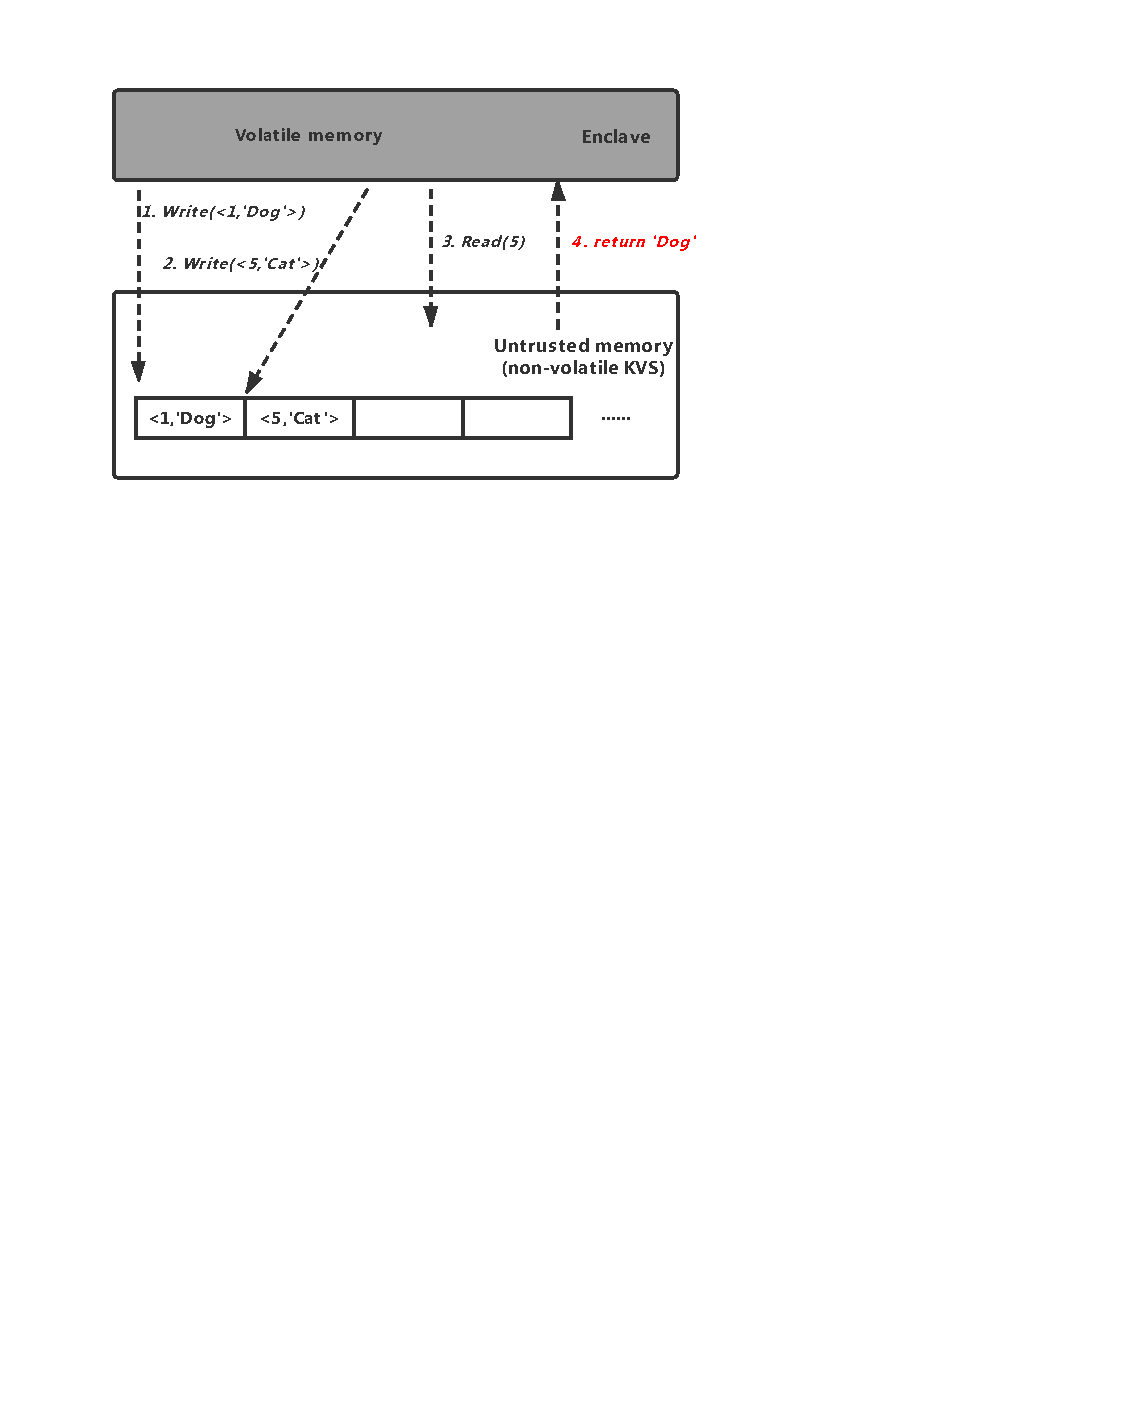
\includegraphics[width=.45\textwidth]{rollback.pdf}
        \caption[title]{An example of rollback attack towards KVS on SGX-enabled host. 
        The malicious OS returns an older version of value in KVS and the trusted enclave (in gray)
        cannot detect it. The records should be sealed/unsealed but we omit these operations for simplicity.}
        % \caption[title]{DAENet's scalability with increasing number of nodes.}
        \label{fig:rollback}
\end{figure}

To formalize, in addition to leverage the protection of SGX, we should also develop a freshness protection 
mechanism to protect against rollback attacks that replay old state of objects. In other word, we aim to expand 
the security protection of SGX from trusted volatile memory of enclaves to untrusted non-volatile memory of 
the outside, even when the system reboot, crash or during migration.

\section{Solutions}
In this section, we mainly introduce three state-of-art solutions in solving the problem we mention in \S\ref{problem}. 
We separately describe their motivation, inner designations, and respective improving directions in detail.

\subsection{SGX Counter}

Intel has recently added support for monotonic counters~(MC)~\cite{} as an optional SGX feature. The Monotonic Counter can be utilized by enclave developers for rollback attack protection. 

\subsubsection{Overview}

SGX supports creating a limited number of MCs for each enclave. Monotonic counters are shared among enclaves that have the same code. An enclave can query availability of counters from the Platform Service Enclave (PSE). If supported, the enclave can create up to 256 counters. The default owner policy encompasses that only enclaves with the same signing key may access the counter. Counter creation operation returns an identifier that is a combination of the Counter ID and a nonce to distinguish counters created by different entities. On creating a MC, it gets written to the non-volatile memory in the platform. The enclave must store the counter identifier to access it later, as there is no API call to list existing counters. After a successful counter creation, an enclave can increment, read, and delete the counter. Because each enclave shares the same value of the monotonic counters, it guarantees the verification for data freshness. In other words, only when an enclave preserves the same counter value as the others in the platform, its reserving data are the latest. Also, when one enclave encounters crash or reboot, it can recover data with the help of monotonic counters shared in the platform. 

According to the SGX API documentation [5], counter operations involve writing to a non-volatile memory. Repeated write operations can cause the memory to wear out, and thus the counter increment operations may be rate limited. Based on Intel developer forums [51], the counter service is provided by the Management Engine on the Platform Control Hub (PCH).


\subsubsection{Limitations}
Though being as a selective feature in SGX architecture, it has strict memory constraints and performs slow during experimental tests~\cite{}. 

The SGX Monotonic Counter updates take 80-250 ms and reads 60-140 ms. When an enclave needs to persistently store an updated state, it can increment a counter, include the counter value and identifier to the sealed data, and verify integrity of the stored data based on counter value at the time of unsealing. However, such approach may wear out the used non-volatile memory. Assuming a system that updates one of the enclaves on the same platform once every 250 ms, the non-volatile memory used to implement the counter wears out after approximately one million writes, making the counter functionality unusable after a couple of days of continuous use. Even with a modest update rate of one increment per minute, the counters are exhausted in two years. Thus, SGX counters are unsuitable for systems where state updates are frequent and continuous. Additionally, since the non-volatile memory used to store the counters resides outside the processor package, the mechanism is likely vulnerable to bus tapping and flash mirroring attacks~\cite{}.

Note that SGX also provides the SGX trusted time feature for checking the timestamp of one stored data record. However, including a timestamp to each sealed data version only allows an enclave to distinguish which out of two seals is more recent, enclaves cannot identify if the sealed data provided by the OS is fresh and latest.






\subsection{ROTE}

To overcome the slowness of SGX Monotonic Counters and provide stable persistent rollback attack protections, ROTE~\cite{} is proposed as a distributed trusted counter service based on a consensus protocol.

\subsubsection{Overview}



\subsubsection{Limitations}




\subsection{Speicher}





% \section{Runtime}
This is runtime.
\section{Evaluation Plan}
This is evaluation part.
\section{Conclusion}
In this report, we discussed the freshness problem in state-of-art Key-Value Store (KVS) 
systems. Typically, so-called rollback attackers might return an older version of records 
to users. The use of Intel SGX helps nullify part of this problem, including the 
confidentiality of data and integrity of execution code. However, directly apply SGX
cannot solve this problem because SGX also fails to check the latest version of records. 
Some prior works develop different counter increment based techniques to protect against
rollback attacks, including ROTE~\cite{matetic2017rote}, Speicher~\cite{bailleu2019speicher}, EnclaveDB~\cite{enclavedb:sp18} and so on.
These systems either incurring moderate overhead or being effective in a distributed setting,
with some drawbacks in either evaluation or crash tolerance. 
Thus, we propose some improvements on the design and evaluation of existing work and plan 
to implement and evaluate our prototype.

%ACKNOWLEDGMENTS are optional
% \section{Acknowledgments}
% This section is optional.
%
% The following two commands are all you need in the
% initial runs of your .tex file to
% produce the bibliography for the citations in your paper.

\newpage
\bibliographystyle{abbrv}
\bibliography{sigproc-sp-csis8101}  % sigproc-sp-csis8101.bib is the name of the Bibliography in this case

% That's all folks!
\end{document}
